\documentclass{standalone}
\usepackage{amsmath,amssymb}
\usepackage{newtxtext,newtxmath}
\usepackage{xcolor}
\usepackage{tikz}
\usetikzlibrary{arrows.meta,positioning,calc,decorations.pathreplacing}

\definecolor{ink}{HTML}{1B1F23}
\definecolor{slate}{HTML}{555E68}
\definecolor{muted}{HTML}{8E96A0}
\definecolor{light}{HTML}{C6CCD2}
\definecolor{faint}{HTML}{E6E9ED}
\definecolor{quantum}{HTML}{2C5E8A}
\definecolor{quantumlight}{HTML}{6C9AC3}
\definecolor{quantumpale}{HTML}{DCE7F2}
\definecolor{ochre}{HTML}{B86B19}
\definecolor{ochrelight}{HTML}{E2B98B}
\definecolor{ochrepale}{HTML}{F6E9D8}

\newcommand{\pfmain}[1]{{\fontsize{7.6}{8.8}\selectfont\color{ink}#1}}
\newcommand{\pfsub}[1]{{\fontsize{7.0}{8.2}\selectfont\color{ink}#1}}
\newcommand{\pfslate}[1]{{\fontsize{7.0}{8.2}\selectfont\color{slate}#1}}
\newcommand{\pfquantum}[1]{{\fontsize{7.0}{8.2}\selectfont\color{quantum}#1}}
\newcommand{\pfochre}[1]{{\fontsize{7.0}{8.2}\selectfont\color{ochre}#1}}

\newcommand{\haty}{%
  \tikz[baseline=(Y.base)]{%
    \node[inner sep=0pt, outer sep=0pt] (Y) {$y$};
    \draw[line width=0.45pt, line cap=round, line join=round]
      ([xshift=0.3pt,yshift=1.25pt]Y.north west) -- ([yshift=2.45pt]Y.north) -- ([xshift=-0.3pt,yshift=1.25pt]Y.north east);
  }%
}

\tikzset{
  pfarrow/.style={-{Stealth[length=3.3pt, width=2.4pt]}, line width=0.65pt, draw=ink},
  pfmutedarrow/.style={-{Stealth[length=3.2pt, width=2.3pt]}, line width=0.60pt, draw=slate},
  pfqgate/.style={
    rectangle, draw=ink, fill=white, line width=0.65pt,
    minimum height=0.225in, inner sep=2.2pt,
    font=\fontsize{7.0}{8.0}\selectfont, text=ink
  }
}

\begin{document}
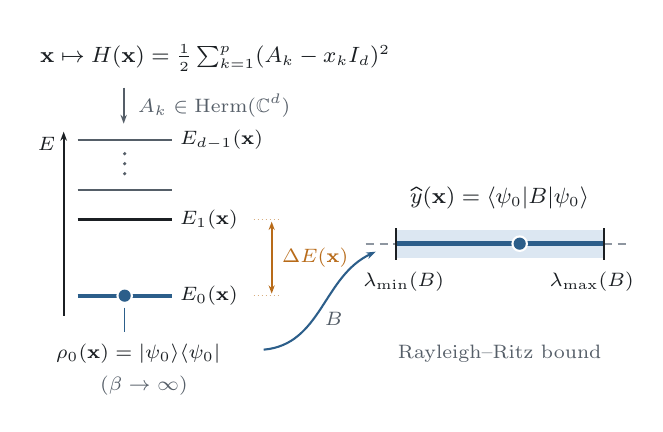
\begin{tikzpicture}[x=1in, y=1in]
  \useasboundingbox (0,0) rectangle (3.0335in, 1.88in);
  \fill[white] (0,0) rectangle (3.0335, 1.88);

  % Error Hamiltonian H(x) = (1/2) sum_k (A_k - x_k I_d)^2 and spectral gap Delta E(x)
  \node[anchor=west, inner sep=0pt] at (0.06, 1.73)
    {\pfmain{$\mathbf{x} \mapsto H(\mathbf{x}) = \tfrac{1}{2}\sum_{k=1}^{p}(A_k - x_k I_d)^2$}};

  \draw[pfmutedarrow] (0.48, 1.58) -- (0.48, 1.40);
  \node[anchor=west, inner sep=0pt] at (0.55, 1.49)
    {\pfslate{$A_k \in \mathrm{Herm}(\mathbb{C}^d)$}};

  \draw[pfarrow] (0.18, 0.44) -- (0.18, 1.36);
  \node[anchor=east, inner sep=0pt] at (0.14, 1.30) {\pfsub{$E$}};

  \draw[quantum, line width=1.45pt] (0.25, 0.54) -- (0.72, 0.54);
  \fill[white] (0.485, 0.54) circle[radius=3.0pt];
  \fill[quantum] (0.485, 0.54) circle[radius=2.2pt];
  \node[anchor=west, inner sep=0pt] at (0.76, 0.54) {\pfsub{$E_0(\mathbf{x})$}};

  \draw[ink, line width=0.90pt] (0.25, 0.92) -- (0.72, 0.92);
  \node[anchor=west, inner sep=0pt] at (0.76, 0.92) {\pfsub{$E_1(\mathbf{x})$}};

  \draw[slate, line width=0.65pt] (0.25, 1.07) -- (0.72, 1.07);
  \foreach \dy in {1.15, 1.20, 1.25} {
    \fill[slate] (0.485, \dy) circle[radius=0.65pt];
  }
  \draw[slate, line width=0.70pt] (0.25, 1.32) -- (0.72, 1.32);
  \node[anchor=west, inner sep=0pt] at (0.76, 1.32) {\pfsub{$E_{d-1}(\mathbf{x})$}};

  \draw[ochre!55, line width=0.45pt, densely dotted] (1.13, 0.54) -- (1.26, 0.54);
  \draw[ochre!55, line width=0.45pt, densely dotted] (1.13, 0.92) -- (1.26, 0.92);
  \draw[ochre, line width=0.75pt, {Stealth[length=3.0pt, width=2.2pt]}-{Stealth[length=3.0pt, width=2.2pt]}]
    (1.22, 0.55) -- (1.22, 0.91);
  \node[anchor=west, inner sep=0pt] at (1.27, 0.73) {\pfochre{$\Delta E(\mathbf{x})$}};

  \draw[quantum, line width=0.55pt] (0.485, 0.48) -- (0.485, 0.36);
  \node[anchor=west, inner sep=0pt] at (0.14, 0.25)
    {\pfsub{$\rho_0(\mathbf{x}) = \lvert\psi_0\rangle\langle\psi_0\rvert$}};
  \node[anchor=west, inner sep=0pt] at (0.36, 0.09)
    {\pfslate{($\beta \to \infty$)}};

  \draw[quantum, line width=0.75pt, -{Stealth[length=3.4pt, width=2.4pt]}]
    (1.18, 0.27) to[out=5, in=205] (1.74, 0.76);
  \node[anchor=north, inner sep=0pt] at (1.53, 0.46) {\pfslate{$B$}};

  % Rayleigh-Ritz spectral readout bound y_hat(x) in [lambda_min(B), lambda_max(B)]
  \node[anchor=center, inner sep=0pt] at (2.36, 1.03)
    {\pfmain{$\haty(\mathbf{x}) = \langle\psi_0\vert B\vert\psi_0\rangle$}};

  \fill[quantumpale] (1.84, 0.73) rectangle (2.88, 0.87);
  \draw[muted, line width=0.60pt, densely dashed] (1.69, 0.80) -- (1.84, 0.80);
  \draw[muted, line width=0.60pt, densely dashed] (2.88, 0.80) -- (3.01, 0.80);
  \draw[quantum, line width=1.65pt] (1.84, 0.80) -- (2.88, 0.80);
  \draw[ink, line width=0.85pt] (1.84, 0.72) -- (1.84, 0.88);
  \draw[ink, line width=0.85pt] (2.88, 0.72) -- (2.88, 0.88);

  \fill[white] (2.46, 0.80) circle[radius=3.0pt];
  \fill[quantum] (2.46, 0.80) circle[radius=2.2pt];

  \node[anchor=north, inner sep=0pt] at (1.88, 0.66) {\pfsub{$\lambda_{\min}(B)$}};
  \node[anchor=north, inner sep=0pt] at (2.82, 0.66) {\pfsub{$\lambda_{\max}(B)$}};
  \node[anchor=center, inner sep=0pt] at (2.36, 0.25)
    {\pfslate{Rayleigh--Ritz bound}};
\end{tikzpicture}
\end{document}
